\section{Benutzerschnittstelle}

\subsection{Einführung}
Die Benutzeroberfläche muss so aufgebaut sein, dass auch unerfahrene \glspl{Benutzer} das System problemlos verwenden können.
Um die Benutzerführung zu optimieren werden insbesondere sog. \glspl{Wizard} verwendet. In diesen wird der Benutzer dann durch die verschiedenen Schritte eines gegebenen Ablaufs geführt. Darüber hinaus wird an vielen Stellen das \gls{Drag-and-Drop}-Konzept verwendet.
Hierdurch wird die Benutzeroberfläche intuitiver und die Dauer der einzelnen Interaktionen des Nutzers mit dem System wird verkürzt.
\subparagraph{}
Alle Angaben zur Benutzeroberfläche sind vorläufig, da auch viele der Wunschkriterien aus Kapitel \ref{subsec:project_goals-wunschkriterien} in dieser Oberfläche realisiert werden. Die exakte visuelle Ausgestaltung der Elemente ist ebenfalls vorläufig.
\subsection{Login}
\begin{figure}[!htb]
	\caption{Loginseite des Systems mit Anmeldung über den \gls{Shibboleth Identity Provider} des \gls{KIT}s}
	\label{fig:gui-login-1}
	\centering
	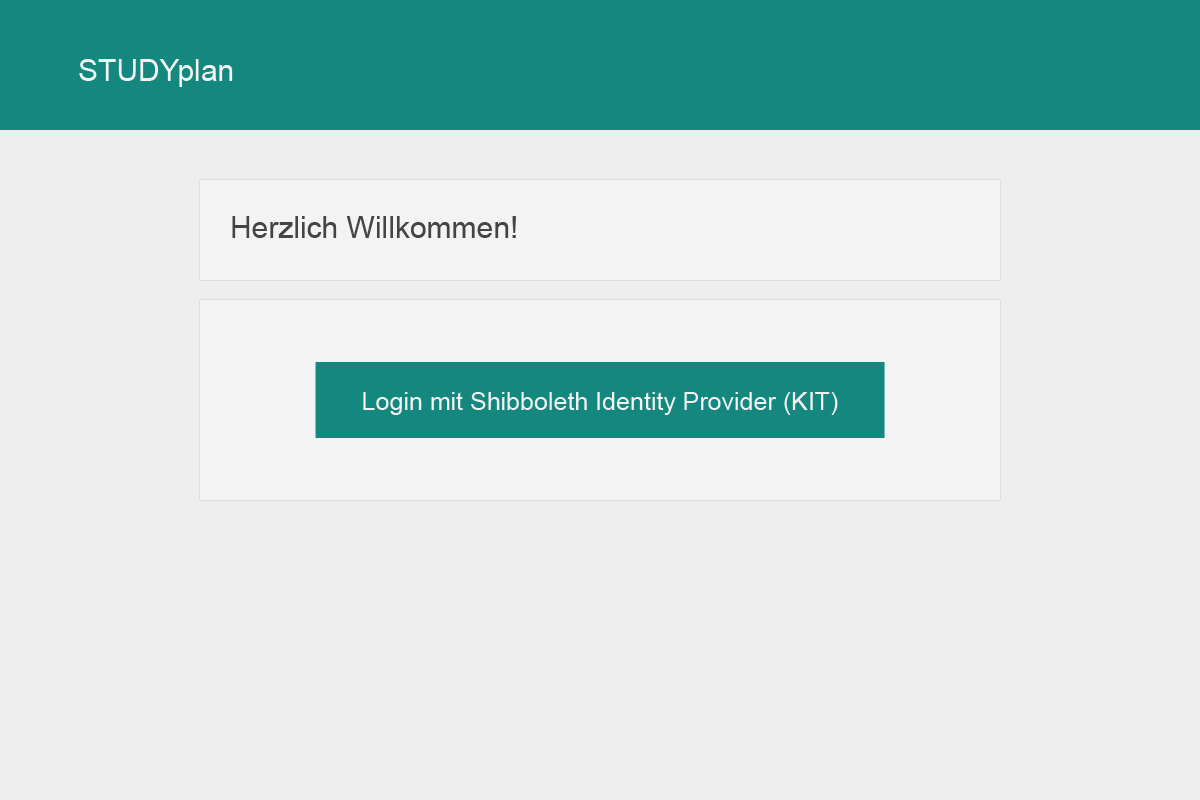
\includegraphics[width=0.7\textwidth]{../GUI/ergebnisse/login-1.png}
\end{figure}
Abbildung \ref{fig:gui-login-1} zeigt die Login-Seite. Diese sollte recht minimalistisch sein und lediglich die Möglichkeit bieten sich mit Hilfe des \gls{Shibboleth Identity Provider}s des \gls{KIT}s einloggen zu können.
\subparagraph{}
Loggt sich der Nutzer zum ersten Mal in das System ein wird er zum Registrierungs-\gls{Wizard} (siehe Kapitel \ref{subsec:gui-registrierung}) weitergeleitet. Wenn er sich bereits zuvor schon einmal eingeloggt hat wird er auf die Hauptseite (siehe Kapitel \ref{subsec:gui-hauptseite}) weitergeleitet.
\subsection{Registrierungs-Wizard}
\label{subsec:gui-registrierung}
Nach dem Login wird man zum Registrierungs-\gls{Wizard}s weitergeleitet. Auf der ersten Seite (Abbildung \ref{fig:gui-registrierung-1}) wird der Nutzer dort nach grundlegenden Informationen wie dem \gls{Studiengang} und dem \gls{Semester des Studienbeginns} gefragt. Die Eingabe dieser Daten ist verpflichtend.
\subparagraph{}
Nachdem der Nutzer dann auf den Pfeil in der unteren Ecke geklickt hat, wird er auf die zweite Seite des \gls{Wizard}s (Abbildung \ref{fig:gui-registrierung-2}) weitergeleitet. Hier kann er angeben, welche \glspl{Modul} er bereits \glslink{Modul begonnen}{begonnen} und/oder \glslink{Modul abgeschlossen}{abgeschlossen} hat. 
Nach dem Bearbeiten der zweiten Seite des \gls{Wizard}s und dem Klick auf den Pfeil, wird der Nutzer auf die Hauptseite des Systems (siehe Kapitel \ref{subsec:gui-hauptseite}) weitergeleitet.
\subparagraph{}
Durch den \gls{Wizard} soll sichergestellt werden, dass der Nutzer alle für das System relevanten Daten (siehe Kapitel \ref{subsec:product_data-benutzerdaten}) eingibt bevor er mit der Nutzung beginnt.
\begin{figure}[!htb]
	\caption{Erste Seite des Registrierungs-\gls{Wizard}s mit Eingabe von Studienfach und Studienbeginn}
	\label{fig:gui-registrierung-1}
	\centering
	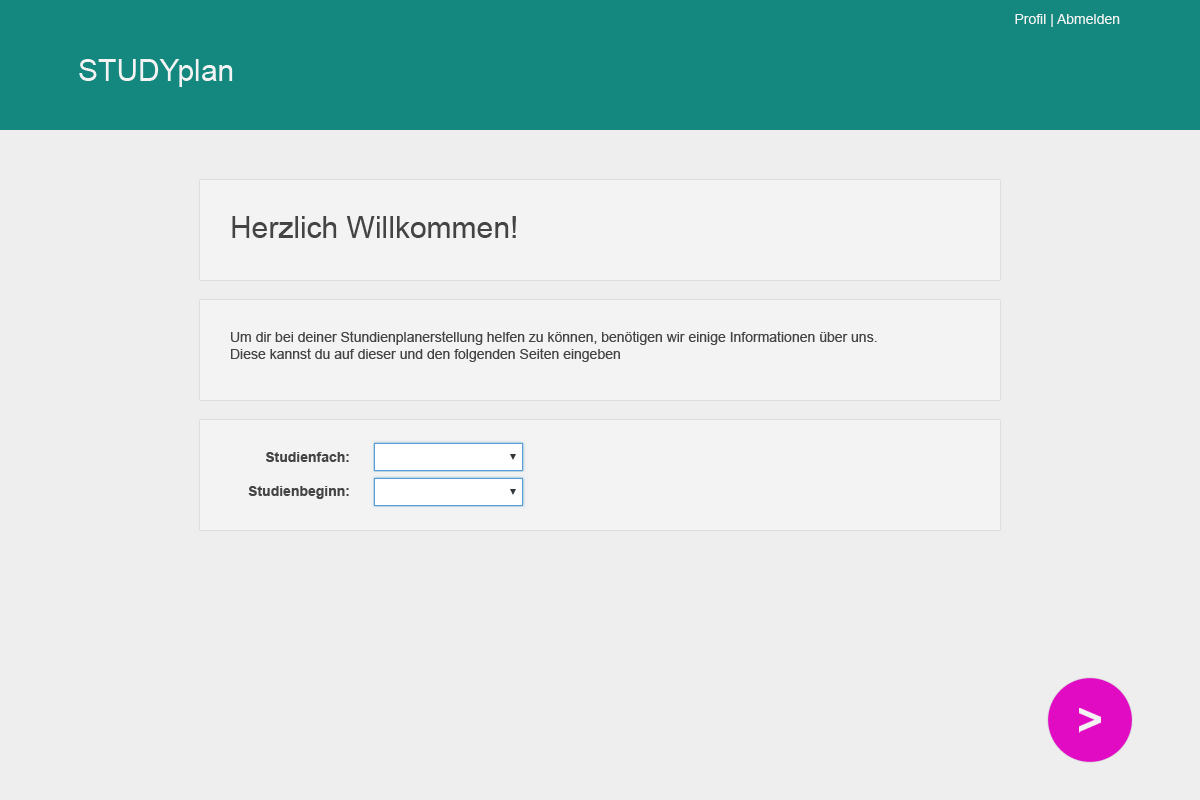
\includegraphics[width=0.7\textwidth]{../GUI/ergebnisse/registrierung-1.png}
\end{figure}

\begin{figure}[!htb]
	\caption{Zweite Seite des Registrierungs-\gls{Wizard}s mit Eingabe der schon begonnenen Module}
	\label{fig:gui-registrierung-2}
	\centering
	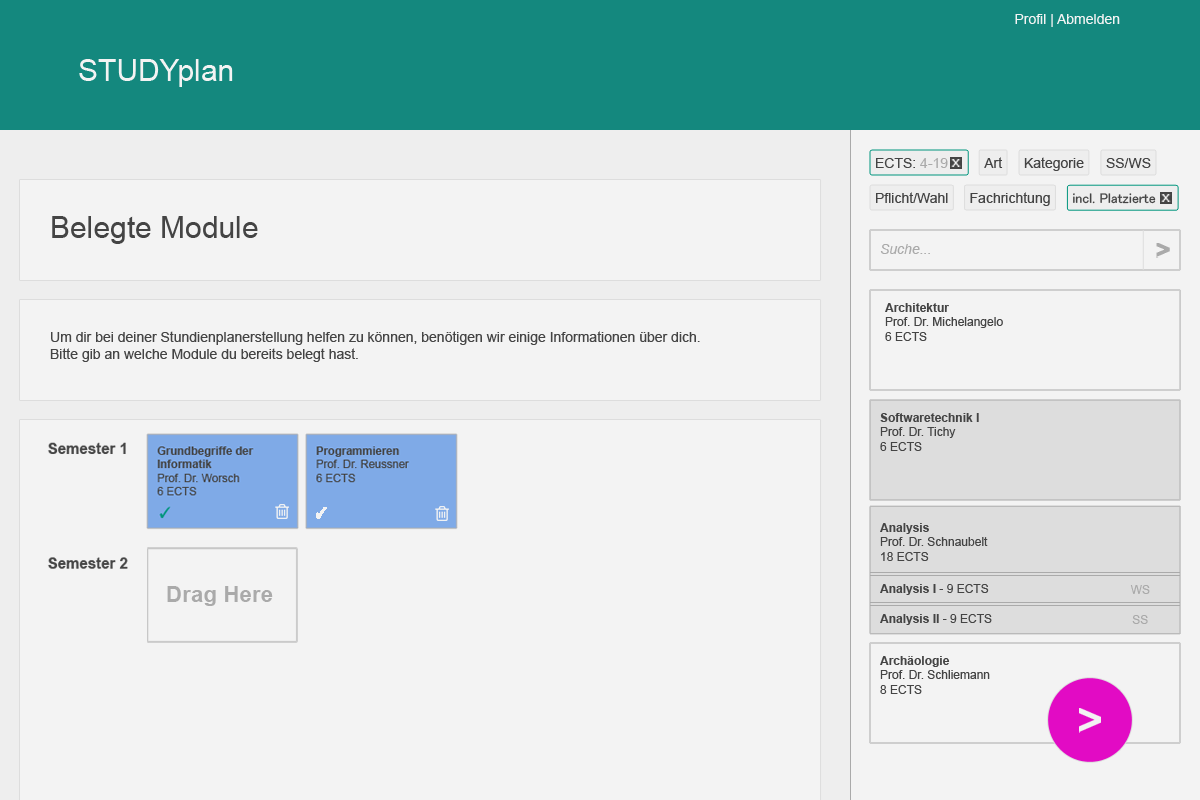
\includegraphics[width=0.7\textwidth]{../GUI/ergebnisse/registrierung-2.png}
\end{figure}


\subsection{Hauptseite}
\label{subsec:gui-hauptseite}
Die Hauptseite des Systems (Abbildung \ref{fig:gui-hauptseite-1}) stellt für den Nutzer die zentrale Anlaufstelle für alle Anwendungsfälle dar. Der Nutzer kann auf dieser Seite seine vorhandenen \glspl{Studienplan} anzeigen, duplizieren, löschen sowie exportieren. Auch sieht der Nutzer über das farbige Icon bereits ob der Plan in seinem jetzigen Zustand verifiziert ist (grün) oder es ein Problem mit dem Plan gibt (rot). Über das selektieren von mehreren Plänen, kann er auch Pläne vergleichen oder mehrere gleichzeitig löschen. Mittels des Plus-Buttons kann er darüber hinaus neue \glspl{Studienplan} erstellen.\newline
Beim Klick auf "Anzeigen" wird der Nutzer auf die Seite zur manuellen Bearbeitung von \glspl{Studienplan} (siehe Kapitel \ref{subsec:gui-manuelle-bearbeitung}) geleitet. Beim Klick auf das "+" wird er nach einem Namen für die Seite gefragt und anschließend ebenfalls auf die Seite zur manuellen Bearbeitung weitergeleitet.
\begin{figure}[!htb]
	\caption{}
	\label{fig:gui-hauptseite-1}
	\centering
	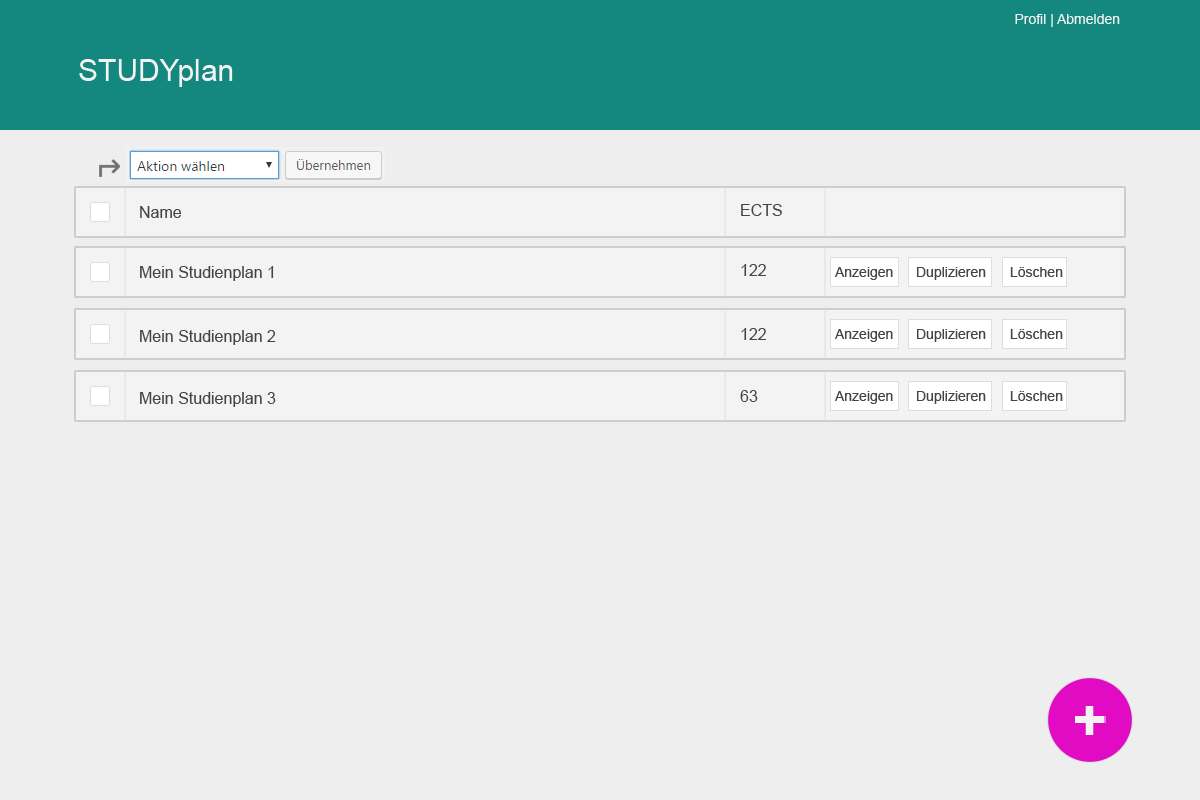
\includegraphics[width=0.7\textwidth]{../GUI/ergebnisse/hauptseite-1.png}
\end{figure}

\subsection{Manuelle Studienplan-Bearbeitung}
\label{subsec:gui-manuelle-bearbeitung}
In dieser Ansicht (Abbildung \ref{fig:gui-bearbeitung-1}) ist es dem Nutzer möglich, seinen \gls{Studienplan} manuell zu bearbeiten. Hierfür kann er mittels \gls{Drag-and-Drop} \glspl{Modul} oder \glspl{Teilmodul} (z.B. das \gls{Teilmodul} Analysis I in der Abbildung) in das gewünschte Semester zu ziehen. Durch das Ziehen wird das \gls{Modul} dem \gls{Studienplan} hinzugefügt. Durch einen Klick auf den Namen des \gls{Studienplan}s kann auch dieser verändert werden.
\subparagraph{Verifizierung}
Mit einem Klick auf "Überprüfen" wird der Plan verifiziert (siehe Kapitel \ref{subsec:gui-verifizierung}).\newline
Ist das Icon neben dem Button gelb wurde der aktuelle Stand des \gls{Studienplan}s noch nicht verifiziert. Ist das Icon rot ist die Verifizierung fehlgeschlagen. Wenn das Icon grün ist war die Verifizierung erfolgreich.
\subparagraph{Generierung}
Mit einem Klick auf den Button "Plan vervollständigen" gelangt man zum "Generierungs-Wizard" (siehe Kapitel \ref{subsec:gui-generierung}). Für die Generierung kann man bereits auf dieser Seite in der Sidebar (mit Hilfe der Pfeil-Buttons) Präferenzen für die Module angeben. Diese werden bei der späteren Generierung berücksichtigt.
\subparagraph{Farbkonvention}
\glspl{Modul} werden in der Sidebar auf der rechten Seite grau sobald sie bereits im \gls{Studienplan} vorhanden sind.\newline
\glslink{Modul begonnen}{Begonnene} \glspl{Modul} werden mit blauem Hintergrund angezeigt.
\glslink{Modul abgeschlossen}{Abgeschlossene} \glspl{Modul} werden mit einem grünen Haken angezeigt.
\begin{figure}[!htb]
	\caption{}
	\label{fig:gui-bearbeitung-1}
	\centering
	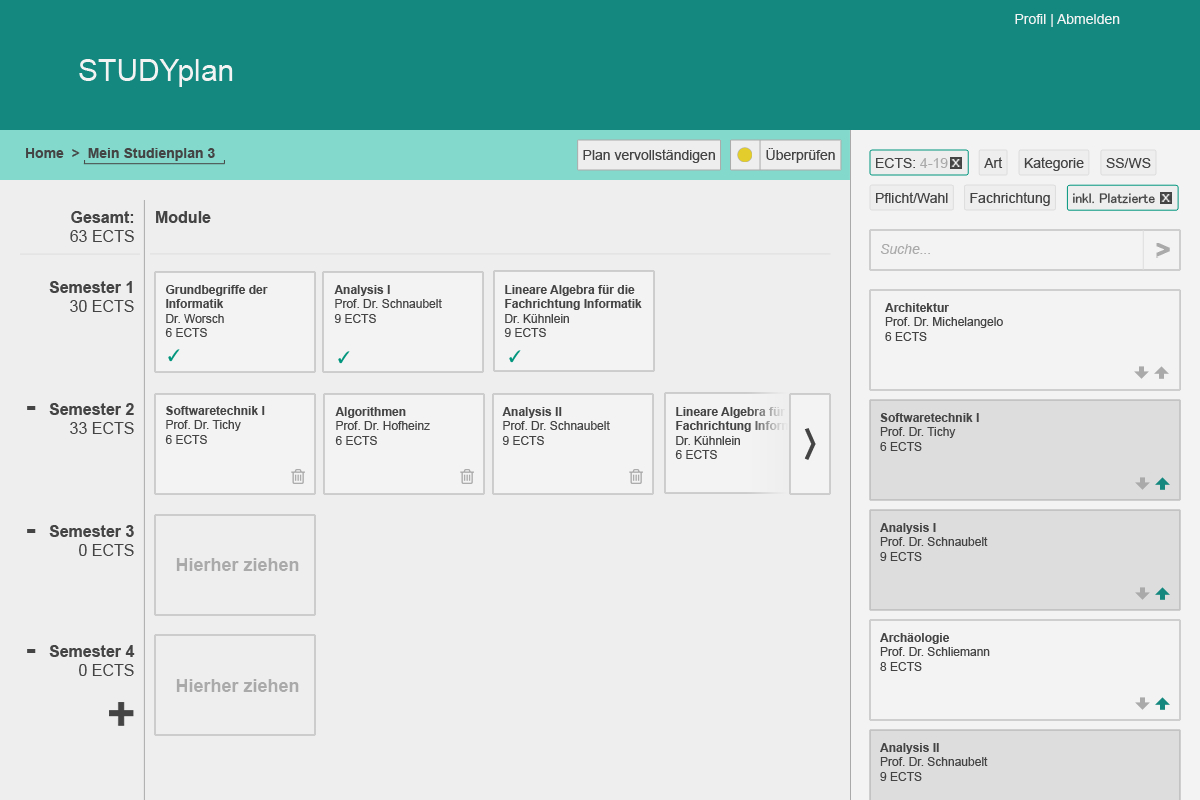
\includegraphics[width=0.7\textwidth]{../GUI/ergebnisse/bearbeitung-1.png}
\end{figure}

\subsubsection{Modul-Sidebar}
\label{subsec:gui-modul-sidebar}
In der Seitenleiste kann man die Module nach verschiedenen Kriterien filtern (Abbildungen \ref{fig:gui-module-filtern-1} und \ref{fig:gui-module-filtern-2}). Hierfür gibt es zum einen vorgefertigte Filter, welche durch Buttons einstellbar sind und zum anderen eine Freitextsuche. Die ausgewählten Filter werden sofort angewendet.
\begin{figure}[!htb]
	\caption{}
	\label{fig:gui-module-filtern-1}
	\centering
	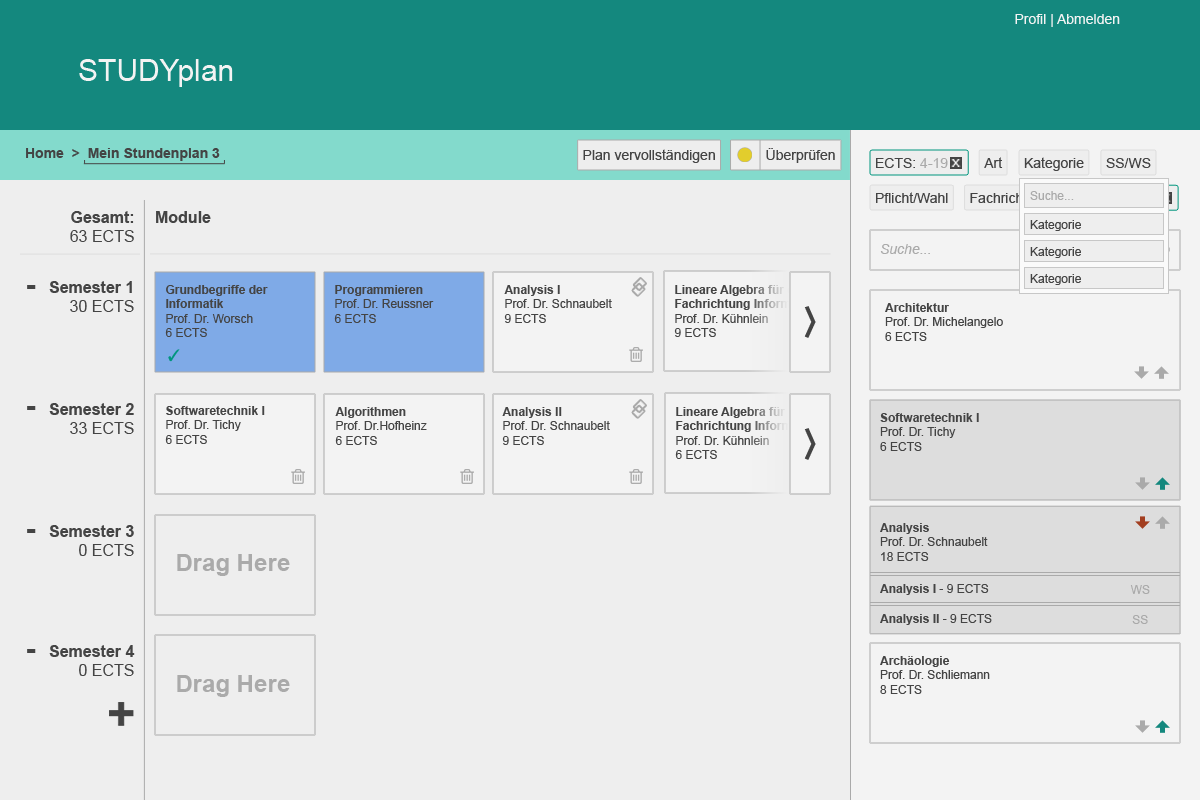
\includegraphics[width=0.7\textwidth]{../GUI/ergebnisse/module-filtern-1.png}
\end{figure}
\begin{figure}[!htb]
	\caption{}
	\label{fig:gui-module-filtern-2}
	\centering
	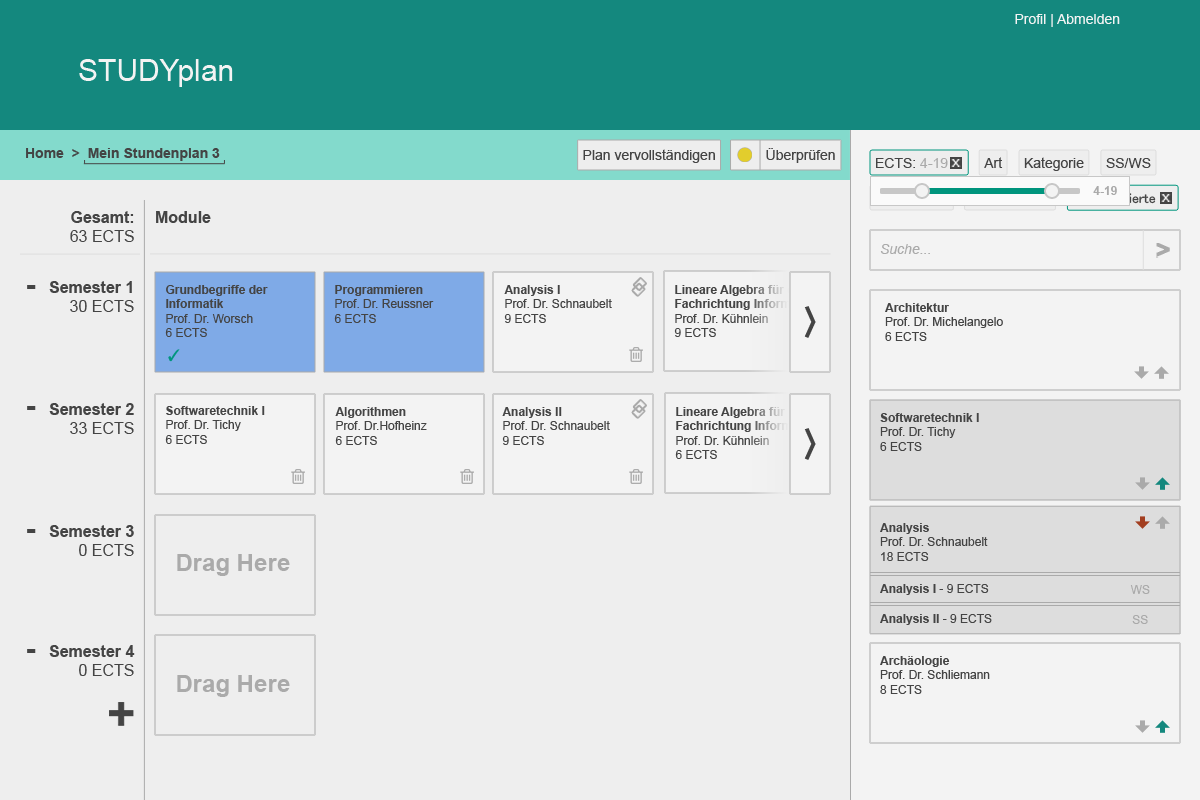
\includegraphics[width=0.7\textwidth]{../GUI/ergebnisse/module-filtern-2.png}
\end{figure}

\subsubsection{Modul-Informationen anzeigen}
Beim Klick auf ein Modul wird die reguläre Modul-Filter-Sidebar unsichtbar (siehe Kapitel \ref{subsec:gui-modul-sidebar}) und es wird stattdessen eine Sidebar mit Informationen über das jeweilige Modul angezeigt (Abbildung \ref{fig:gui-modul-info-1}).
\begin{figure}[!htb]
	\caption{}
	\label{fig:gui-modul-info-1}
	\centering
	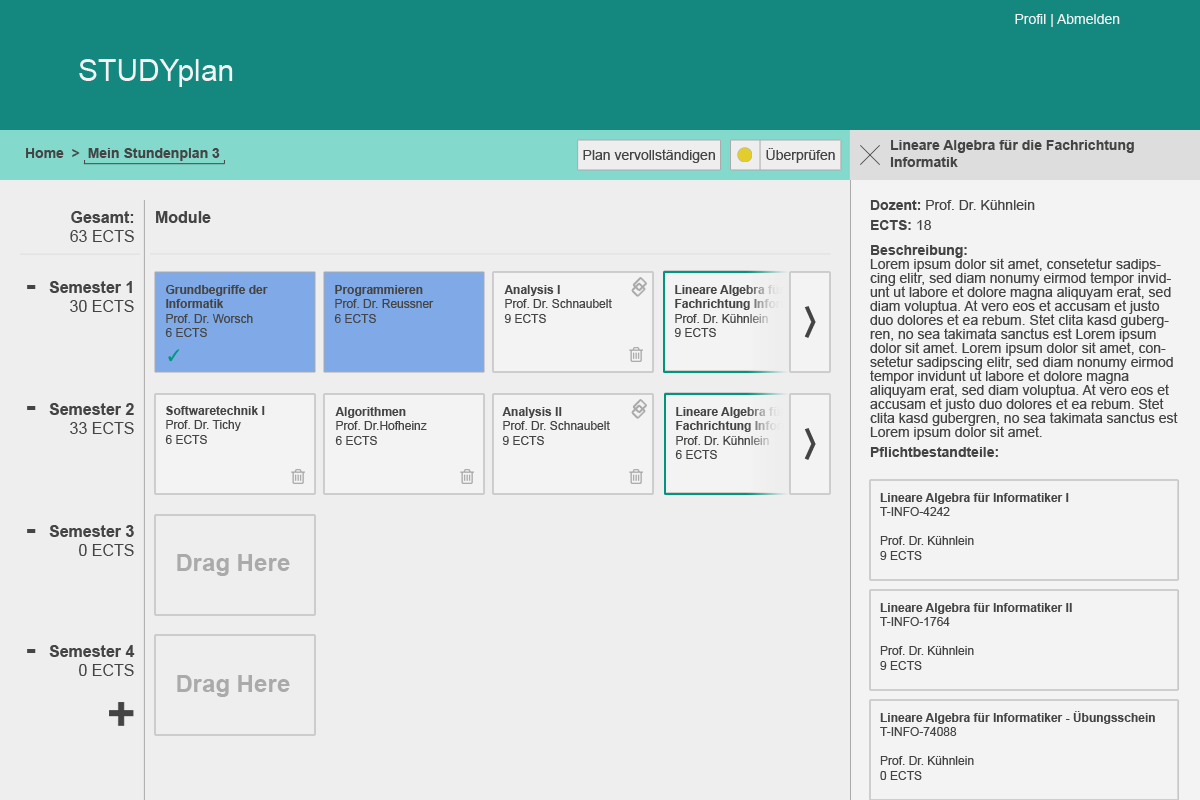
\includegraphics[width=0.7\textwidth]{../GUI/ergebnisse/modul-info-1.png}
\end{figure}


\subsection{Generierungs-Wizard}
\label{subsec:gui-generierung}
Bei der Studienplan-Generierung wir der \gls{Benutzer} zunächst nach den Zielen des Studienplans gefragt (Abbildung \ref{fig:gui-generierung-1}). Anschließend kann er Präferenzen für \glspl{Modul} angeben (Abbildung \ref{fig:gui-generierung-2}). Auf der darauffolgenden Seite werden noch einige vom Ziel des Studienplans abhängige Fragen gestellt (Abbildung \ref{fig:gui-generierung-3}). Anschließend wird dann der generierte Studienplan angezeigt (Abbildung \ref{fig:gui-generierung-4}). Hier hat der \gls{Benutzer} die Wahl den Plan zu verwerfen, zu übernehmen oder unter einem anderen Namen zu speichern.
\begin{figure}[!htb]
	\caption{}
	\label{fig:gui-generierung-1}
	\centering
	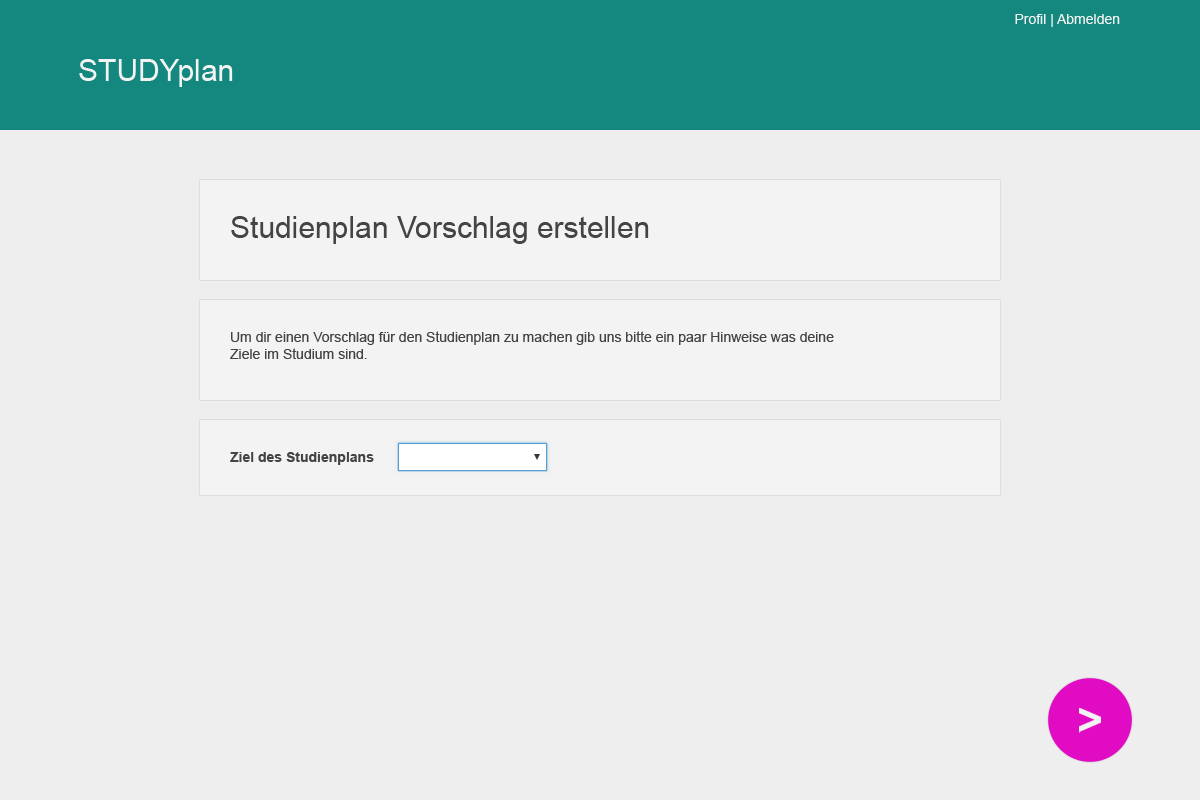
\includegraphics[width=0.7\textwidth]{../GUI/ergebnisse/generierung-1.png}
\end{figure}

\begin{figure}[!htb]
	\caption{}
	\label{fig:gui-generierung-2}
	\centering
	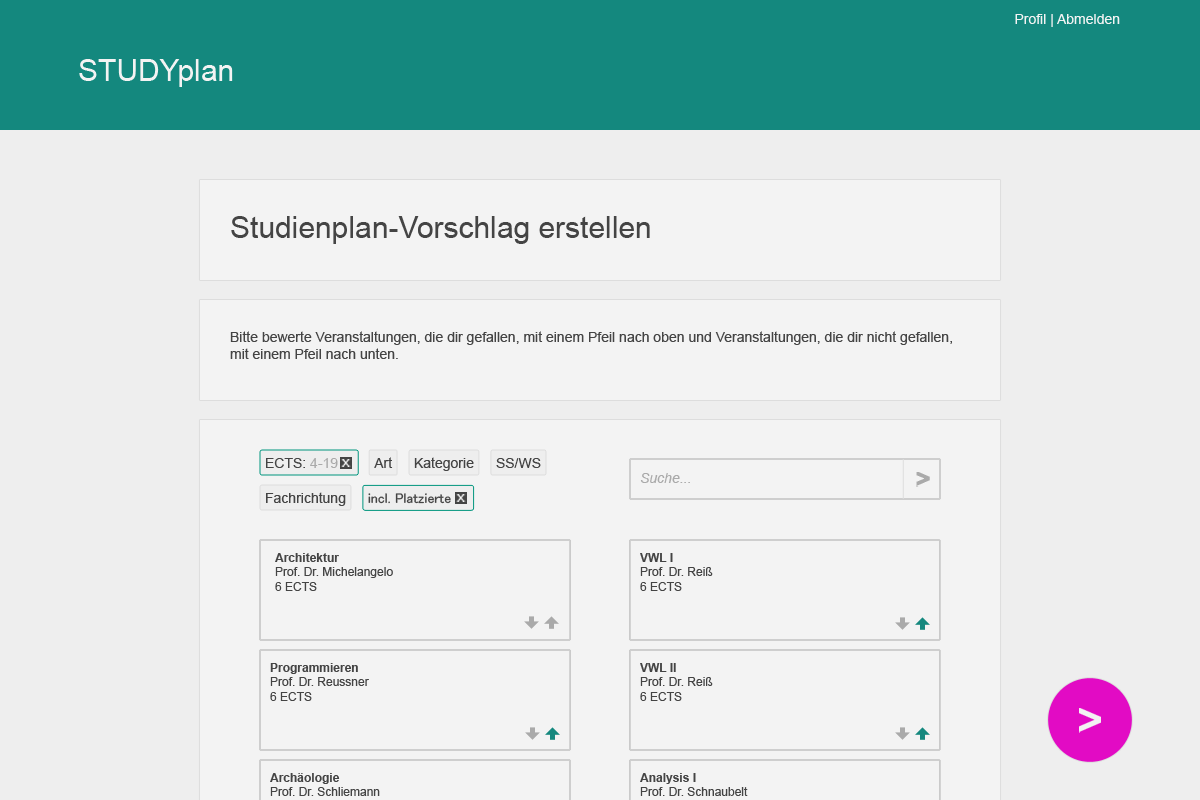
\includegraphics[width=0.7\textwidth]{../GUI/ergebnisse/generierung-2.png}
\end{figure}

\begin{figure}[!htb]
	\caption{}
	\label{fig:gui-generierung-3}
	\centering
	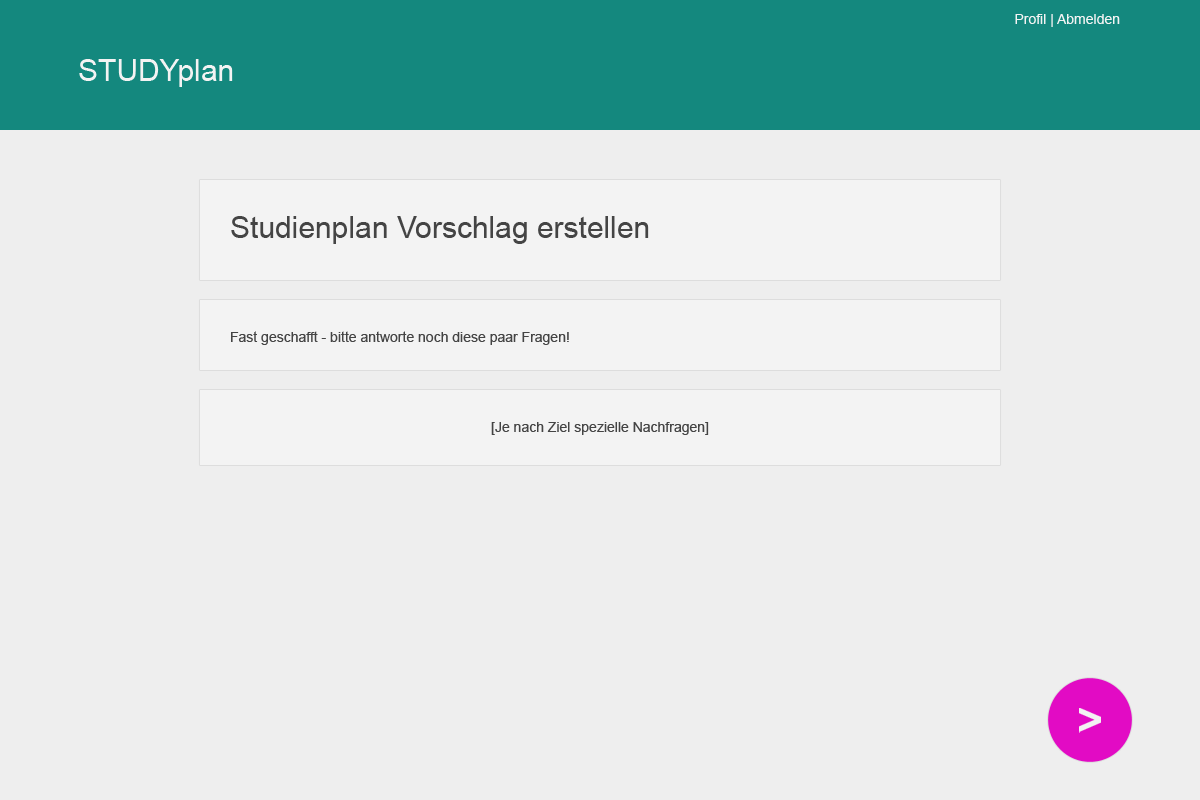
\includegraphics[width=0.7\textwidth]{../GUI/ergebnisse/generierung-3.png}
\end{figure}

\begin{figure}[!htb]
	\caption{}
	\label{fig:gui-generierung-4}
	\centering
	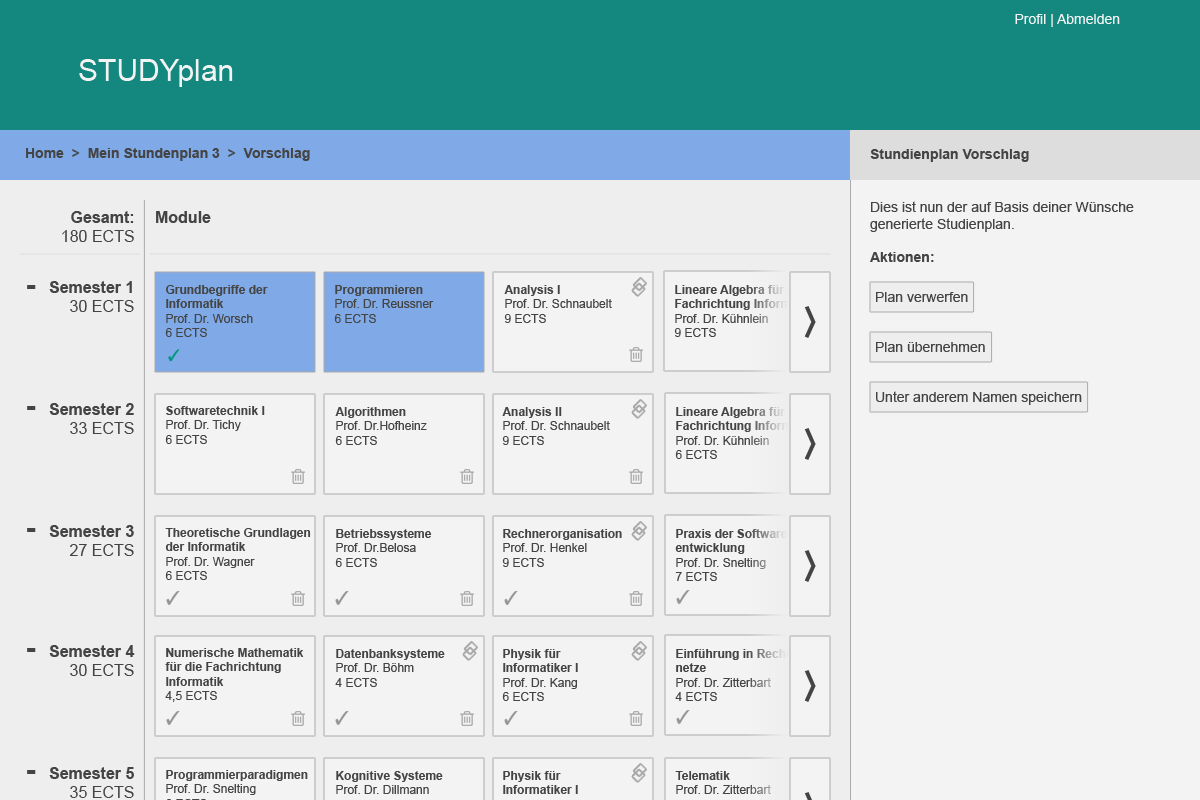
\includegraphics[width=0.7\textwidth]{../GUI/ergebnisse/generierung-4.png}
\end{figure}

\subsection{Verifizierung}
\label{subsec:gui-verifizierung}
Nach einem Klick auf den Button "Überprüfen" wird die Verifizierung im Hintergrund durchgeführt.\newline
Schlägt die Verifikation fehl (Abbildung \ref{fig:gui-verifizierung-2}), bekommt der \gls{Benutzer} eine Benachrichtigung in der unteren rechten Ecke angezeigt. Das Icon neben "Überprüfen" wird rot und die \glspl{Modul}, welche in dieser Form nicht belegt werden können erhalten einen roten Rahmen.\newline
Ist die Verifikation erfolgreich (Abbildung \ref{fig:gui-verifizierung-1}), erscheint ein grünes Icon neben dem Button "Überprüfen" und der \gls{Benutzer} erhält ebenfalls eine Benachrichtigung in der unteren rechten Ecke.
\begin{figure}[!htb]
	\caption{}
	\label{fig:gui-verifizierung-1}
	\centering
	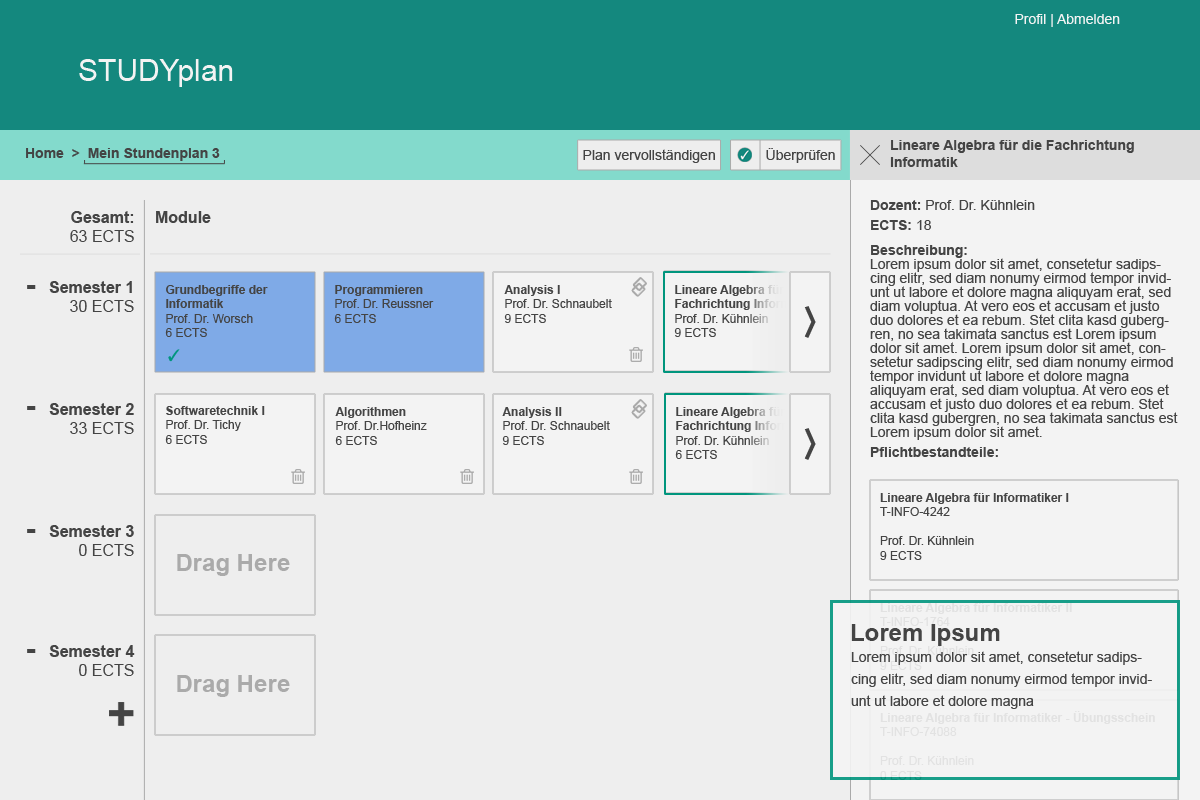
\includegraphics[width=0.7\textwidth]{../GUI/ergebnisse/verifizierung-1.png}
\end{figure}
\begin{figure}[!htb]
	\caption{}
	\label{fig:gui-verifizierung-2}
	\centering
	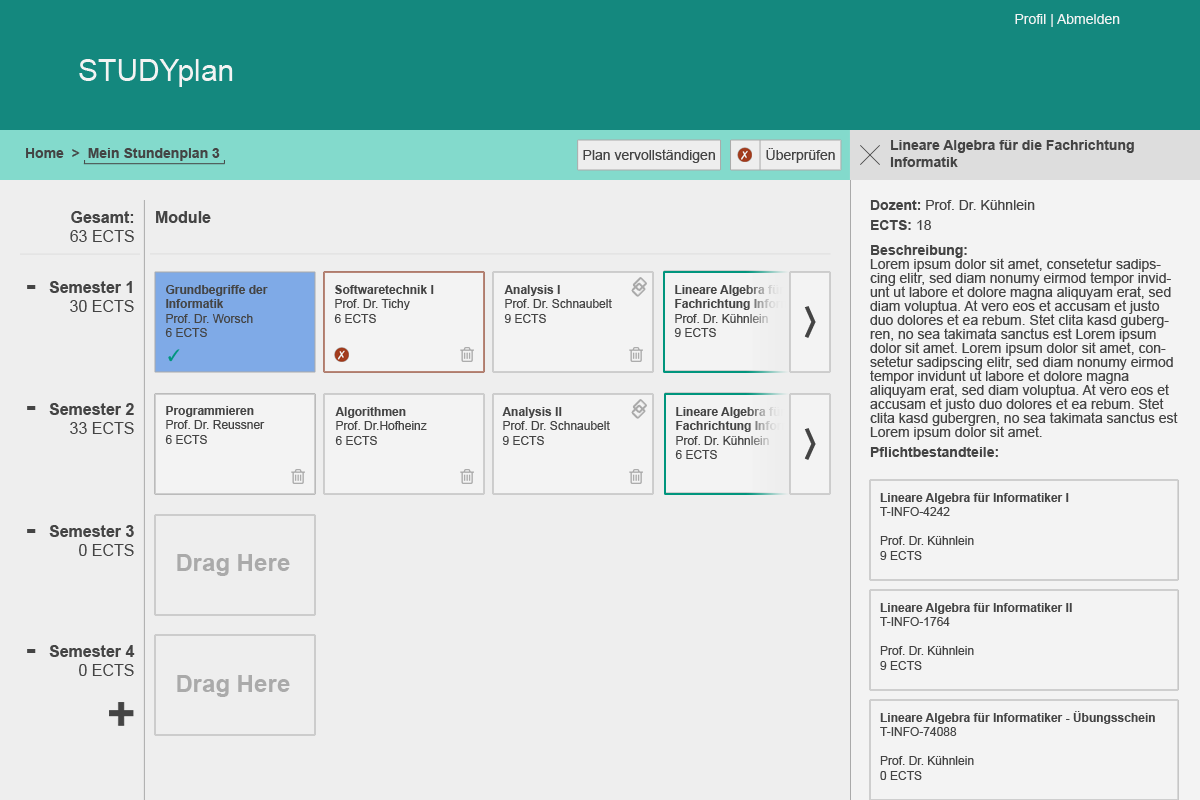
\includegraphics[width=0.7\textwidth]{../GUI/ergebnisse/verifizierung-2.png}
\end{figure}

\subsection{Profil}
Im Profil (Abbildung \ref{fig:gui-profil-1}) ist es dem Benutzer möglich, seine bisher \glslink{Modul begonnen}{begonnenen} und \glslink{Modul abgeschlossen}{abgeschlossenen} \glspl{Modul} zu bearbeiten.
\begin{figure}[!htb]
	\caption{}
	\label{fig:gui-profil-1}
	\centering
	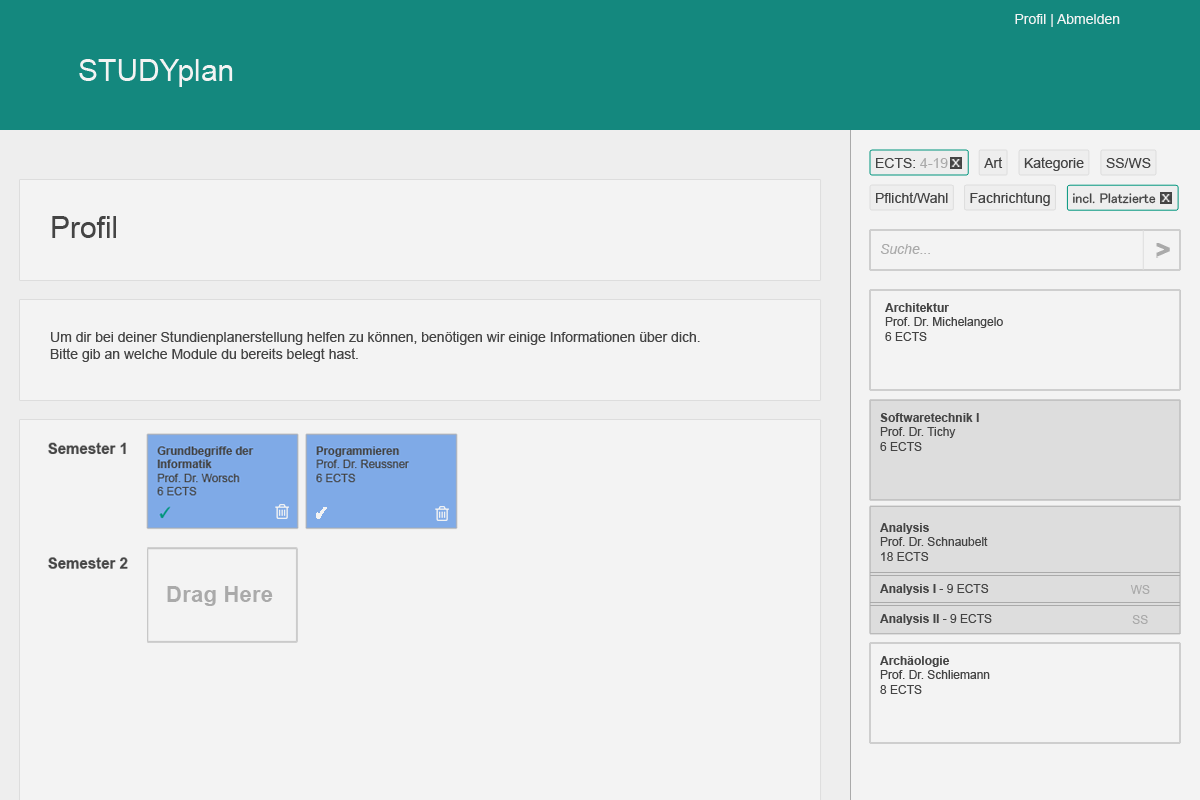
\includegraphics[width=0.7\textwidth]{../GUI/ergebnisse/profil-1.png}
\end{figure}